% % % % % % % % % % % % % % % % % % % % % % % % % % % % % % % % % % % % % % % % %
\section{Freie Theoreme}
% % % % % % % % % % % % % % % % % % % % % % % % % % % % % % % % % % % % % % % % %

\label{sec:freie-theoreme}

In der Einleitung wurde bereits kurz thematisiert, dass man allein durch Betrachten der Typsignatur einer Funktion bereits
eine grundlegende, intuitive Vorstellung davon erhalten kann, welche Funktionalität sich ungefähr hinter dieser Funktion
verbirgt. Haskells Typsystem sorgt dafür, dass Funktionen in ihren Implementierungsmöglichkeiten
teilweise stark eingeschränkt sind. Der Grund hierfür ist der parametrische Polymorphismus, der in Haskellfunktionen
mit freien Typvariablen Anwendung findet. Nicht nur verringert das Typsystem die Fehleranfälligkeit von produziertem
Code, es vereinfacht auch Rückschlüsse auf die Funktionsweise und Korrektheitsbeweise.

Außerdem wurde bereits angedeutet, dass es eine Möglichkeit gibt, systematisch Theoreme zu gegebenen Typsignaturen
herzuleiten. Diese sogenannten \textit{freien Theoreme}, ihre Herleitung und ihre Verwendung sind Thema dieses Kapitels.
Zunächst wird an einem Beispiel
erläutert, wie die Vorgehensweise intuitiv zu erklären ist. Der darauf folgende Abschnitt behandelt die formale Herleitung
eines freien Theorems zu einer beliebigen Typsignatur nach Wadler \cite{wadler}.

Daraufhin wird die Erweiterung des Vorgehens um Typkonstruktorklassen thematisiert, wie sie
auch verwendet wird von Voigtländer in \cite{voigtlander}. Am Ende des Kapitels wird schließlich an einem
praktischen Beispiel gezeigt, wie ein freies Theorem für einen Beweis verwendet werden kann.

%Wie in der Einleitung bereits angedeutet wurde, lässt sich diese Intuition in Formeln ausdrücken. In diesem Abschnitt
%wird erklärt, wie diese so genannten freien Theoreme aussehen. Es wird erläutert, wie man sie herleitet und warum
%das möglich ist. Am Ende des Abschnittes wird insbesondere darauf eingegangen, welche Rolle Typkonstruktorklassen
%für die Generierung von freien Theoremen spielen.

%Einleitend wurde bereits das mächtige Typsystem Haskells angesprochen. Dieses Typsystem ist komplett statisch und
%unterstützt parametrischen Polymorphismus, wie in den Grundlagen erläutert wurde. Nicht nur verringert ein solches Typsystem
%die Fehleranfälligkeit von produziertem Code, es vereinfacht auch Rückschlüsse auf die Funktionsweise und Korrektheitsbeweise.
%In dieser Arbeit geht es vor allem um die bereits angesprochenen freien Theoreme. Diese lassen sich herleiten, ohne dass man
%überhaupt die konkrete Implementierung in Betracht ziehen muss. Man nennt sie ``freie Theoreme'', weil man sie gewissermaßen
%``geschenkt'' bekommt. Wie genau man diese Theoreme herleitet, soll in diesem Abschnitt genauer erläutert werden.


% - - - - - - - - - - - - - - - - - - - - - - - - - - - - - - - - - - - - - - - - - - - - - - - - - - - - - - - - - - - - - - - - - - - - - - - - - - - - - -
\subsection{Beispiel}
% - - - - - - - - - - - - - - - - - - - - - - - - - - - - - - - - - - - - - - - - - - - - - - - - - - - - - - - - - - - - - - - - - - - - - - - - - - - - - -

Bevor die theoretische Herangehensweise beschrieben wird, bietet es sich zunächst an, die Vorgehensweise intuitiv an einem
Beispiel zu erklären. Dabei werden noch keine Definitionen eingeführt oder Formeln aufgestellt, es geht vielmehr darum,
ein Gefühl dafür zu vermitteln, warum es überhaupt möglich sein soll, Theoreme allein aus der Signatur eines Ausdrucks
abzuleiten. Im nächsten Abschnitt wird dieses Vorgehen dann konkretisiert und für beliebige Typsignaturen verallgemeinert.

%Als Beispiel soll die folgende Haskell-Typsignatur dienen.
Als einfaches Beispiel dient die Funktion mit der folgenden Typsignatur.

%Zunächst bietet es sich an, die Vorgehensweise an einem konkreten Beispiel vorzuführen. Bevor es um die theoretische
%Herangehensweise geht, soll das Vorgehen erst einmal intuitiv motiviert werden. Wir betrachten die folgende Haskell-Funktion.

\begin{align}
f :: [a] \rightarrow [a] \label{eq:fsig}
\end{align}

Gegeben ist also eine Funktion $f$, die von einer Liste auf eine Liste abbildet. Das Besondere an dieser Funktion ist, dass sie
nicht für einen konkreten Typ wie beispielsweise $[Integer] \rightarrow [Integer]$ deklariert ist, sondern dass man sie für jeden
beliebigen Typ instanziieren kann, indem man die Typvariable $a$ durch einen Typausdruck einsetzt. Die Funktion ist also für
einen beliebigen Typ deklariert, es handelt sich um eine \textit{polymorphe Funktion}.

Bei der Typvariable $a$ handelt es sich erst einmal um eine ungebundene, \textit{freie} Variable. Man kann sich aber einen impliziten
Allquantor vor der eigentlichen Signatur denken. Tatsächlich existiert dieser Allquantor sogar explizit als Schlüsselwort \texttt{forall} in Haskell,
im Normalfall wird es jedoch nicht explizit benötigt und deshalb meistens weggelassen. Immer, wenn
freie Typvariablen in einer Signatur vorkommen, lässt sich diese Signatur also \textit{schließen}, indem für jede freie Typvariable
ein entsprechender Allquantor an den Anfang gesetzt wird.

Die Instanziierung einer polymorphen Funktion auf einen konkreten Typ wird im weiteren Verlauf der Arbeit beschrieben, indem der
polymorphe Ausdruck mit einem Index versehen wird, der dem Typ entspricht, auf den der Ausdruck instanziiert wird.
$f_{Integer}$ ist dann beispielsweise die Funktion $f$, konkretisiert auf den Typ Integer, d.h. es wird Integer
für $a$ in die Funktionssignatur eingesetzt. $f_{Bool \rightarrow Bool}$ wäre folglich die gleiche Funktion instanziiert auf den Typ
$Bool \rightarrow Bool$, sie hätte also die Signatur $[Bool \rightarrow Bool] \rightarrow [Bool \rightarrow Bool]$.

Hat die Funktion mehrere verschiedene Typvariablen, so werden die einzelnen Typen
in der Reihenfolge des Auftretens der zu ersetzenden Typvariablen angegeben. Eine Funktion mit der Signatur \texttt{g :: a -> b} instanziiert man
folglich mit $g_{Integer\ String}$ auf den Typ $Integer \rightarrow String$.

%Instanziierung einer polymorphen Funktion auf einen bestimmten Typ wird im Folgenden
%durch eine Index-Schreibweise dargestellt. $f_{Integer}$ wäre also eine Funktion mit dem Typen $[Integer] \rightarrow [Integer]$,
%$f_{Bool}$ wäre die gleiche Funktion für den Typen $[Bool] \rightarrow [Bool]$.
%3sie für jeden beliebigen Typen,
%der für die Typvariable a eingesetzt werden
%kann. Es handelt sich also um eine polymorphe Funktion.

Ein entscheidendes Detail bei polymorphen Funktionen in Haskell ist die Art des Polymorphismus.
Man unterscheidet zwischen Ad-Hoc Polymorphismus und parametrischem Poly\-mor\-phis\-mus \todo{cite}. Bei Typvariablen
in Haskell handelt es sich um parametrischen Polymorphismus, das heißt die entsprechende Funktion arbeitet für sämtliche
eingesetzten Typen nach demselben Prinzip.

Erst einmal klingt das nicht besonders außergewöhnlich, es zieht aber wichtige
Konsequenzen mit sich. ``Dasselbe Prinzip'' heißt hier nämlich, dass unabhängig vom eingesetzten Typ die gleichen
Berechnungen stattfinden. Die Funktion kann nicht einmal
durch Fallunterscheidung ermitteln, um welchen konkreten Typ es sich im jeweiligen Fall handelt.
%In diesem Fall handelt es sich um parametrischen Polymorphismus, d.h. die Funktion arbeitet für sämtliche Typen nach dem gleichen Prinzip.

Das ist deswegen etwas Besonderes, weil es dadurch ermöglicht wird, allgemeine Aussagen zu treffen, die für sämtliche
Typinstanziierungen gelten. Vergleicht man diese Methode mit der zweiten Art von Polymorphismus, dem \textit{Ad-Hoc-Polymorphismus},
wird der Vorteil klar: Unter Letzterem versteht man, dass eine Funktion zwar für verschiedene Typen definiert wird, diese jedoch
jeweils eine konkrete, typspezifische Implementierung haben.

Es handelt sich also technisch gesehen um verschiedene Funktionen, die sich einen Namen teilen können, weil anhand der Typsignatur
und der Typen der Parameter, mit denen die Funktion aufgerufen wird, entschieden werden kann, welche der Funktionen jeweils gemeint ist.
Ein Beispiel für Ad-Hoc-Polymorphismus bietet die Programmiersprache \textit{C++}: Hier ist es möglich, mehrere Funktionen mit gleichem
Namen in einer Klasse zu deklarieren, solange sie unterschiedliche Signaturen besitzen, wie das folgende Beispiel zeigt.

\begin{minted}{cpp}
class Log
{
public:
   void log(TextObject* t);
   void log(Image* t);
   void log(Test* t);
}
\end{minted}

Hier werden drei Methoden deklariert, die alle den Namen \texttt{log} haben, sich jedoch durch den Typ des Parameters
unterscheiden. Die jeweilige Implementierung, die hier nicht zu sehen ist, kann sich von Funktion zu Funktion komplett unterscheiden.
Auch Haskell bietet mit sogenannten \texttt{Typklassen} Ad-Hoc-Polymorphismus. Darauf wird später noch genauer eingegangen.

Beim Ad-Hoc-Polymorphismus kann also jede Funktion eine eigene Implementierung haben, außerdem ist jeder Funktion
bekannt, auf welchem Typ sie arbeitet, was es ihr ermöglicht, typspezifische Operationen anzuwenden. Es liegt nahe, dass dies
allgemeingültige Aussagen über solche Funktionen unmöglich macht.

%Die Implementierungen können also komplett unterschiedlich funktionieren und kennen den konkreten Typen, für de%n sie
%implementiert sind, können also auf typspezifische Eigenschaften zugreifen. Man kann sich denken, dass das allgemeine Aussagen
%unmöglich macht.

Wir betrachten wieder die Beispielfunktion $f$ aus (\ref{eq:fsig}). Durch parametrischen Polymorphismus ist sie also für jeden beliebigen
Typ $a$ definiert. Das hat Konsequenzen für die Funktionsweise dieser Funktion.

Man kann sich an dieser Stelle die Frage stellen: Wie kann die Funktion die Liste erzeugen, die sie zurückgeben muss? Sie kennt den konkreten Typ nicht,
das heißt sie kann keine neuen Elemente ``erfinden'', weil sie keine Informationen darüber hat, welchen Typ die Listenelemente haben müssen.
Und Ausdrücke, die zu jedem beliebigen Typ passen, gibt es in Haskell
nicht\footnote{Tatsächlich kann man undefinierte Werte als Ausdrücke ansehen, die zu einem beliebigen Typ generiert werden können --
diese werden jedoch erst einmal außen vor gelassen. In Kapitel \ref{sec:striktheit-und-rekursion} wird etwas genauer darauf eingegangen.}.
Eine Möglichkeit hat sie aber dennoch: Sie kann die Elemente der Eingabeliste wiederverwenden.
Die einzige Möglichkeit für die Funktion, die Liste zu ändern, besteht also in einer Umsortierung der Listenelemente.

Doch auch für eine Neusortierung der Liste hat die Funktion wenige Anhaltspunkte. Sie kennt zwar die Länge der Liste, doch ohne Kenntnis des Typen kann sie keine weiteren Aussagen über den Inhalt der einzelnen Listenelemente treffen (und da die Klasse Eq
nicht gegeben ist, nicht mal über deren Gleichheit). Auch hat sie aufgrund der referenziellen Transparenz %\todo{kann man das hier einfach so einstreuen?}
in Haskell keinen globalen Kontext oder ähnliches, anhand dessen sie Entscheidungen treffen könnte.
Sie wird also gezwungenermaßen je zwei Listen gleicher Länge stets gleich behandeln.
%Sie wird also für zwei Listen gleicher Länge $l$ und $l'$ exakt das Gleiche tun.

In der Einleitung wurde bereits die Haskell-Funktion \texttt{map} eingeführt, die eine Funktion auf jedes Element einer Liste
anwendet und eine Liste gleicher Länge zurückgibt, in dem jedes Element durch die Eingabefunktion manipuliert wurde.

%Bevor weiter argumentiert werden kann, soll an dieser Stelle eine bekannte Funktion aus Haskell eingeführt werden. Die Funktion
%\texttt{$map :: (a \rightarrow b) \rightarrow [a] \rightarrow [b]$} erwartet eine Funktion als ersten Parameter und eine Liste als
%zweiten Parameter. Sie erzeugt aus der Liste eine neue Liste gleicher Länge, indem jedes Element mit der übergebenen Funktion in
%ein neues Element überführt wird.

Haskell verwendet für Funktionsapplikation das Prinzip des Currying, das heißt, dass eine Funktion mit $n$ Parametern, die auf ein
Argument angewandt wird, eine neue Funktion zurückgibt, in der dieses Argument fest gesetzt ist, die also nur noch $n-1$ Parameter erwartet. \todo{quote}
Man kann die die $map$-Funktion also auch anders interpretieren: $map$, angewandt auf eine Funktion, gibt eine Funktion zurück, die
die Funktionalität der Eingabefunktion für Listen bietet, sie also in den Listen-Kontext \textit{liftet}.
%Da Haskells Funktionsapplikation das Prinzip des Currying verwendet, \todo{quote?} kann man diese Funktion auch auf eine andere
%Weise interpretieren: $map$, angewandt auf eine Funktion, \textit{liftet} diese in den Listen-Kontext, gibt also eine Funktion zurück,
%die dieselbe Funktionalität für Listen bietet.

Im Folgenden nehmen wir an, dass die Funktion $f$ auf einen beliebigen konkreten Typ instanziiert wurde.
Wir betrachten jetzt eine beliebige nicht-polymorphe Funktion $g$, die auf diesem konkreten Typ arbeitet. $map\ g$ liefert folglich eine Funktion,
die $g$ auf sämtliche Elemente einer Eingabeliste
anwendet. Jede Liste, die durch Anwendung von $map\ g$ entsteht, wird die gleiche Anzahl an Elementen haben wie die ursprüngliche Liste.
Darüber hinaus vertauscht $map\ g$ die Listenelemente nicht, jedes neue Element wird an derselben Stelle stehen wie
sein Ursprungselement.

Auf dieser Argumentation aufbauend kann man erkennen, dass es unerheblich für die Ergebnisliste ist, ob man zuerst die
Funktion $f$ auf eine Liste appliziert und dann auf die resultierende Liste die Funktion $map\ g$ anwendet, oder ob man
in umgekehrter Reihenfolge vorgeht. Abbildung \ref{fig:fmapg} veranschaulicht dies für eine Beispielfunktion $f$, die Listen
umkehrt, und eine Funktion $g$, die zu jedem Listenelement den Wert $1$ hinzuaddiert. Hervorgehoben ist die Position
eines Elements in dieser Liste. Im linken Teil der Abbildung wird zunächst die Funktion $f$ appliziert und als zweites
$map\ g$, im rechten Teil wird $map\ g$ zuerst angewendet und dann erst $f$.

\begin{figure}[ht]
\centering
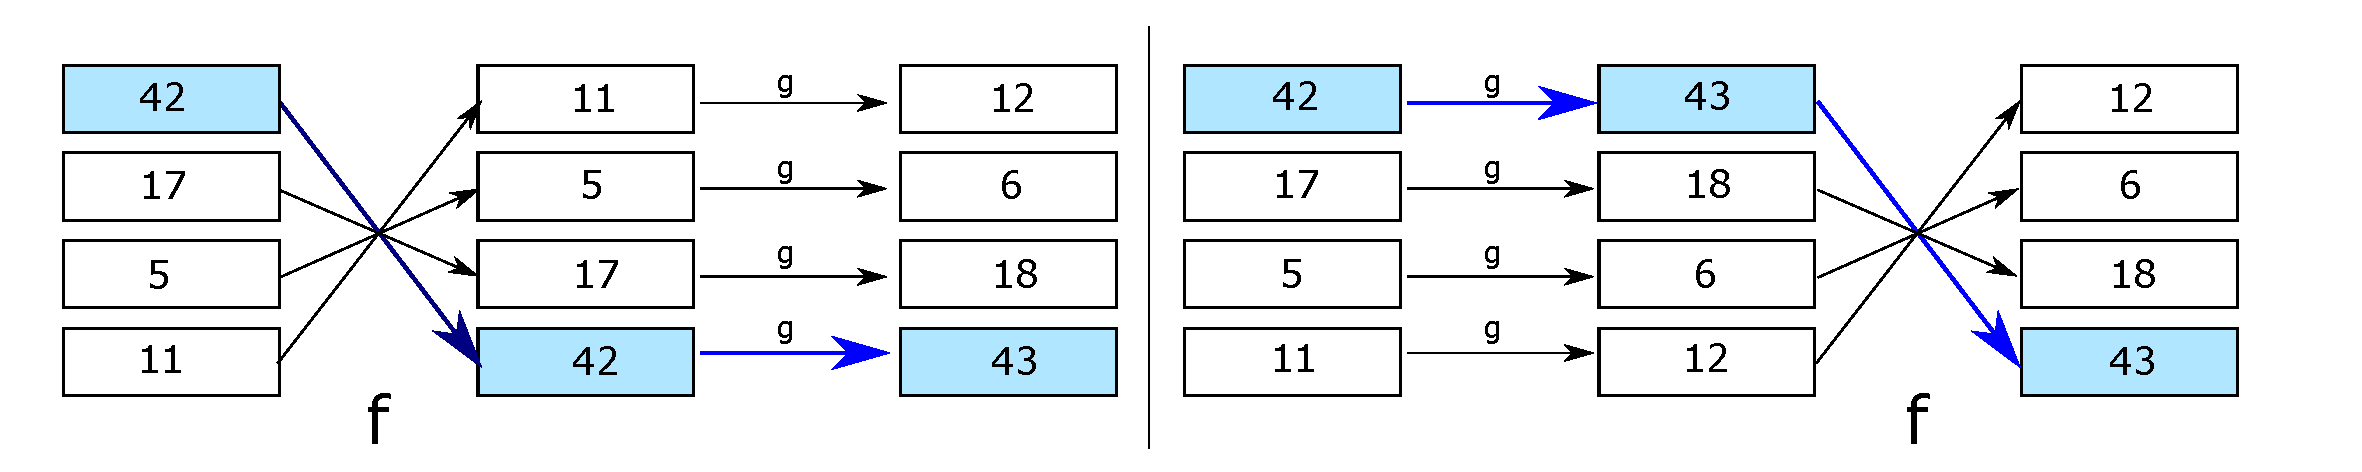
\includegraphics[width=430px]{fmapg}
\caption{Die Reihenfolge der Anwendung von $f$ und $map\ g$ spielt keine Rolle für die Ergebnisliste.}
\label{fig:fmapg}
\end{figure}

%Die folgende Formel fasst diese Aussage mathematisch zusammen.
Die folgende Formel fasst die Aussage der obigen Argumentation als mathematische Aussage zusammen.


%Die Haskell-Funktion \texttt{$map :: (a \rightarrow b) \rightarrow [a] \rightarrow [b]$} wendet eine Funktion auf jedes Element einer Liste an und gibt die resultierende Liste zurück. Da Haskell Currying für Funktionsapplikation verwendet, kann man
%diese Funktion auch auf eine andere Weise interpretieren: $map$, angewandt auf eine Funktion, liftet diese in den Listen-Kontext,
%gibt also eine Funktion zurück, die dieselbe Funktionalität für Listen bietet. Betrachten wir nun eine beliebige Funktion $g :: a \rightarrow a$. Es lassen sich jetzt Aussagen über $map\ g$, angewandt auf Listen, treffen. Zum einen wird jede Liste, auf die man $map\ g$ anwendet, die gleiche Länge haben wie vorher - das liegt einfach in der Natur von $map$.

%Darüber hinaus müssen jeweils zwei Elemente, die an der gleichen Position stehen, auf die gleiche Weise entstanden sein, nämlich
%durch Anwenden von $g$ auf das entsprechende Listenelement.
%Es ist nun logisch, dass es egal ist, ob man zuerst die Funktion f auf eine Liste anwendet und dann die Funktion g auf die
%resultierende Liste mappt, oder ob man in umgekehrter Reihenfolge vorgeht.

\begin{align*}
f (map\ g\ l) = map\ g\ (f\ l)
\end{align*}

Diese Aussage ist ein Theorem, das für beliebige Funktionen g und beliebige Listen l gilt. Doch nicht nur das: Überlegt man sich
einmal, anhand welcher Informationen diese Schlussfolgerung getroffen wurde, wird klar: Das einzige Wissen, das für diese Herleitung
benötigt wurde, ist die Typsignatur der Funktion $f$. Insbesondere wurde die Funktion nicht auf einen konkreten Typ instanziiert,
die Aussage gilt für beliebige Typen -- sie gilt sogar für beliebige Funktionen mit der Typsignatur $[a] \rightarrow [a]$.

%Wir haben für
%die Herleitung kein Wissen über die konkrete Implementierung der Funktion f benötigt; das einzig Bekannte war die Typsignatur.
%Das Theorem gilt also insbesondere für alle Funktionen mit der Typsignatur $[a] \rightarrow [a]$. Da man dieses Theorem
%aus der Typsignatur gwissermaßen ``geschenkt'' bekommt, nennt man es auch ``freies Theorem''.

Natürlich war die vorangegangene Herleitung sehr unkonkret und nicht wirklich mathematischer Natur. Im Folgenden wird dieser
intuitive Ansatz nun mathematisch konkretisiert.
%Daher soll im Folgenden
%erklärt werden, wie man freie Theoreme im Allgemeinen und vor allem auf mathematischer Grundlage herleitet.


% - - - - - - - - - - - - - - - - - - - - - - - - - - - - - - - - - - - - - - - - - - - - - - - - - - - - - - - - - - - - - - - - - - - - - - - - - - - - - -
\subsection{Parametrizität}
% - - - - - - - - - - - - - - - - - - - - - - - - - - - - - - - - - - - - - - - - - - - - - - - - - - - - - - - - - - - - - - - - - - - - - - - - - - - - - -

\label{sec:free-theorems-param}

Der Schlüssel zur Herleitung von freien Theoremen liegt in der Betrachtung von Typen.
Intuitiv werden Typen häufig als Mengen aufgefasst. So würde man den Typ \texttt{Bool} beispielsweise als Menge $\mathbb{B}$
der booleschen Werte auffassen mit $\mathbb{B} = \{ tt, ff \}$, der Typ \texttt{Integer} wäre die Menge der ganzen Zahlen
$\mathbb{Z}$ usw. Komplexere Typen ergeben sich dann durch Zusammensetzung aus einzelnen Basistypen, beispielsweise
würde man den Typen \texttt{$Integer \rightarrow Integer$} auffassen als die Menge $(\mathbb{Z} \rightarrow \mathbb{Z})$ aller Funktionen von den ganzen Zahlen in die ganzen Zahlen.

Die grundsätzliche Idee hinter freien Theoremen basiert auf der Erkenntnis von Reynolds, dass die Semantik eines beliebigen
Ausdrucks verwandte Umgebungen auf verwandte Werte abbildet \cite{reynolds}. Dieses Theorem, von Reynolds das
\textit{Abstraktionstheorem} genannt, wird von Wadler umformuliert zum sogenannten \textit{Parametrizitätstheorem} \cite{wadler},
das diese Erkenntnis für polymorphe Funktionssignaturen nutzbar macht und die Herleitung von Theoremen ermöglicht --
vorausgesetzt, die Typen werden als Relationen aufgefasst statt als Mengen.

Um Typen als Relationen aufzufassen, definiert man sogenannte \textit{relationale Aktionen}, mit denen zu jedem Typ eine entsprechende Relation
konstruiert werden kann \cite{johann2006}.

\begin{mydef}[Relationale Aktion]
Zu jedem n-stelligen Typkonstruktor wird eine Abbildung definiert, die aus $n$ Relationaldarstellungen eine neue Relation konstruiert.
Diese Abbildung nennt man relationale Aktion.
%Eine relationale Aktion ist eine map ??, die eine Anzahl 
\end{mydef}

%das im Folgenden erläutert werden soll. Entscheidend ist, dass man Typen nicht als Mengen sondern als Relationen ausdrückt,
%um dieses Theorem anwenden zu können.

%Für die Herleitung von freien Theoremen ist diese Repräsentation nicht ganz ausreichend, da sie spätestens bei polymorphen
%Typen auf beweistechnische Probleme stößt \todo{?}. Daher greift man auf eine etwas andere Repräsentation zurück: Man
%betrachtet Typen als Relationen.

%Man kann zu einem Typen nun systematisch eine Relation konstruieren, die diesen Typen repräsentiert. Dazu geht man
%folgendermaßen vor:

Man kann also zu einem beliebigen Typ eine Relation konstruieren, die diesen Typ repräsentiert, indem man zu jedem Typkonstruktor
die entsprechende relationale Aktion anwendet. Die einzelnen Relationen werden folgendermaßen konstruiert \cite{voigtlander}.

\begin{itemize}
\item Zu jedem Basistyp $T$ (Int, Bool, etc.) ist die zugehörige Relation die Identitätsrelation $\mathcal{R} = \{ (x, x) | x \in T\}$.
\item Sind $\mathcal{R} : R_1 \Leftrightarrow R_2$ und $\mathcal{S} : S_1 \Leftrightarrow S_2$ Typrelationen, so ist $\mathcal{R} \rightarrow \mathcal{S} = \{ (f, g) | f \in (R_1 \rightarrow R_2), g \in (S_1 \rightarrow S_2), \forall x \in R_1, y \in R_2: (f\ x, g\ y) \in \mathcal{S} \}$ die zugehörige Funktionstyprelation.
\item Ist $\mathcal{F}(\mathcal{X})$ eine Typrelation, die von einer Typrelation $\mathcal{X}$ abhängt, dann definiert man
$\forall \mathcal{X} . \mathcal{F}(\mathcal{X}) = \{ (x, y) | \forall A_1, A_2 \in Typen, \mathcal{A} : A_1 \Leftrightarrow A_2: 
(x_{A_1}, y_{A_2}) \in \mathcal{F}(\mathcal{A}) \}$. Hierbei sind $x$ und $y$ polymorphe Ausdrücke, die durch $x_{A_1}$ und
$y_{A_2}$ auf einen bestimmten Typ instanziiert werden.
\end{itemize}

%Zudem lassen sich bestimmte Typkonstruktoren, wie beispielsweise der Listenkonstruktor $[a]$, durch Lifting der betreffenden
%Relation umsetzen. Man kann beispielsweise für eine gegebene Typrelation $\mathcal{R} : T_1 \Leftrightarrow T_2$ folgenes
%Lifting definieren.

Auch für Datentypen lassen sich Relationen konstruieren. Ein Beispiel ist der Listentypkonstruktor \texttt{[]}, für den man folgende
relationale Aktion definiert, wenn eine Typrelation $\mathcal{R} : T_1 \Leftrightarrow T_2$ gegeben ist.

\begin{align*}
[\mathcal{R}] = \{ ([], []) \} \cup \{ (a : as, b : bs) | (a, b) \in \mathcal{R}, (as, bs) \in [\mathcal{R}] \}
\end{align*}

Andere Standardtypkonstruktoren lassen sich auf ähnliche Weise beschreiben. Nun haben wir die Mittel, zu jeder vorhandenen
Typsignatur eine Relation zu konstruieren. Eine entscheidende Erkenntnis von \cite{wadler}, aufbauend auf
\cite{reynolds}, ist nun das Parametrizitätstheorem. Hierzu muss noch der Begriff \textit{geschlossener Term} definiert werden.

\begin{mytheorem}[Parametrizität]
Ist t ein geschlossener Term von Typ T und $\mathcal{T}$ die zugehörige konstruierte Typrelation, dann gilt $(t, t) \in \mathcal{T}$.
\end{mytheorem}

Ein Term ist dabei geschlossen, wenn er keine freien Variablen enthält.
%folgende: Ist t ein geschlossener Term von Typ T und $\mathcal{T}$ die zugehörige konstruierte
%Typrelation, dann gilt $(t, t) \in \mathcal{T}$ (dieser Satz wird von \cite{wadler} auch Parametrizität, \textit{Parametricity}, genannt).
Damit ist alles gegeben, was man zur Herleitung des freien Theorems benötigt. Wir untersuchen wieder das Beispiel
$f :: [a] \rightarrow [a]$. Durch Parametrizität ist gegeben:

\begin{align*}
(f, f) \in \forall \mathcal{R} . [\mathcal{R}] \rightarrow [\mathcal{R}]
\end{align*}

%Dabei ist zu bemerken, dass in Haskellsyntax typischerweise die Allquantifizierung über die Typvariable weggelassen wird.
Es wurde bereits zu Beginn des Kapitels erwähnt, dass freie Typvariablen in Signaturen mit einem impliziten Allquantor
quantifiziert werden, weshalb hier die entsprechende relationale Aktion Anwendung findet.
%Implizit ist $[a] \rightarrow [a]$ aber gleichbedeutend mit $\forall a . [a] \rightarrow [a]$.
Wir können nun Schritt für Schritt die Definitionen der einzelnen Relationskonstruktionen anwenden, wodurch die Formel
abgerollt wird:

\begin{align*}
&\forall A_1, A_2 \in Typen, \mathcal{A} : A_1 \Leftrightarrow A_2: \\
&(f_{A_1}, f_{A_2}) \in [\mathcal{A}] \rightarrow [\mathcal{A}] \\
& \\
\Leftrightarrow &
\forall A_1, A_2 \in Typen, \mathcal{A} : A_1 \Leftrightarrow A_2: \\
& \forall (l, l') \in [\mathcal{A}]: \\
&(f_{A_1} l, f_{A_2} l') \in [\mathcal{A}] \\
& \\
\Leftrightarrow &
\forall A_1, A_2 \in Typen, \mathcal{A} : A_1 \Leftrightarrow A_2: \\
& \forall (l, l') \in lift_{[]}(\mathcal{A}): \\
& (f_{A_1} l, f_{A_2} l') \in lift_{[]}(\mathcal{A}) \\
\end{align*}

%Zur Erinnerung: $\mathcal{A} : A_1 \Leftrightarrow A_2$ bedeutet, dass $\mathcal{A}$ eine Relation auf den Mengen $A_1$ und $A_2$ ist.

An diesem Punkt haben wir eine Aussage über beliebige Typrelationen $\mathcal{A}$, anschaulicher wäre aber eine Aussage
über beliebige Funktionen. Da man Funktionen als Spezialfall von Relationen betrachten kann, können wir die Aussage
spezifizieren für den Fall, dass es sich bei $\mathcal{A}$ um eine Funktion handelt. Wir quantifizieren dazu statt
über alle Relationen $\mathcal{A} : A_1 \Leftrightarrow A_2$ über alle Funktionen $g : A_1 \rightarrow A_2$.

%Wie in den Grundlagen erläutert wurde, kann man eine Allquantifizierung über Relationen spezialisieren auf Funktionen,
%das heißt wir können uns auf alle $g : A_1 \rightarrow A_2$ beschränken.
%Eine Funktion $f : S \rightarrow T$ kann man auch betrachten als Relation $\{ (x, f x) | x \in S \}$. Anders gesagt: Ist
%$\mathcal{F} : T_1 \Leftrightarrow T_2$ eine Relation zu einer Funktion f, dann gilt für alle $(x, y) \in \mathcal{F}: f x = y$.
%Schränken wir also unsere Aussage auf Funktionen ein, können wir über alle Funktionen $g : A_1 \rightarrow A_2$ quantifizieren. 
Aus dem abgerollten Parametrizitätstheorem haben wir ja bisher die Aussage abgeleitet, dass für alle Parameter $l, l' \in lift_{[]}(\mathcal{A})$
die Aussage $(f_{A_1} l, f_{A_2} l') \in lift_{[]}(\mathcal{A})$ gilt. Als Funktion geschrieben heißt das, es gilt folgende Aussage.

\begin{align*}
lift_{[]}(g) (f_{A_1}\ l) = f_{A_2}\ l'
\end{align*}

Das Lifting von Funktionen in den Listenkontext ist nun ganz einfach das Mapping dieser Funktionen auf Listen, sprich: die Haskell-Funktion
$map$, angewandt auf die entsprechende Funktion.

\begin{align*}
map\ g\ (f_{A_1}\ l) = f_{A_2}\ l'
\end{align*}

Hierbei ist zu bemerken, dass nun nicht mehr über alle Paare $(l, l') \in lift_{[]}(\mathcal{A})$
quantifiziert werden muss, da es zu jedem $l \in [A_1]$ nur genau ein $l' \in [A_2]$ geben kann, für das gilt $map\ g\ l = l'$. Folglich kann man die Variable $l'$
weglassen und stets den Ausdruck $map\ g\ l$ verwenden.
%Da $(l, l') \in [A]$, können wir $l'$ auch anders ausdrücken als $map\ g\ l = l'$. Man erhält also:
Ersetzt man die Variable $l'$ also entsprechend, so erhält man die folgende Aussage.

\begin{align*}
map\ g\ (f_{A_1} l) = f_{A_2} (map\ g\ l)
\end{align*}

Und man erkennt: Es handelt sich um die gleiche Aussage, die wir vorher intuitiv konstruiert haben. Jetzt haben wir bewiesen,
dass sie gültig ist, da Parametrizität gilt. Und ein Theorem dieser Art lässt sich für jede beliebige Typsignatur herleiten.


% - - - - - - - - - - - - - - - - - - - - - - - - - - - - - - - - - - - - - - - - - - - - - - - - - - - - - - - - - - - - - - - - - - - - - - - - - - - - - -
\subsection{Typkonstruktorklassen und -variablen}
% - - - - - - - - - - - - - - - - - - - - - - - - - - - - - - - - - - - - - - - - - - - - - - - - - - - - - - - - - - - - - - - - - - - - - - - - - - - - - -

\label{sec:typkonstruktorklassen}

Die bisherige Theorie basierte auf \cite{wadler} und sah kein Auftreten von Typklassen oder Typkonstruktorklassen vor.
Es wurde angegeben, wie beispielsweise der Listendatentyp in eine Relationaldarstellung überführt werden kann. Ähnliches
ist für beliebige Datentypen möglich, beispielsweise $Maybe$.

Dass in Typsignaturen aber nicht nur über Typvariablen, sondern auch über Variablen allquantifiziert werden kann, die
ihrerseits nicht Platzhalter für spezielle Typen, sondern für Typkonstruktoren sind, wurde bisher außer Acht gelassen. In diesem
Abschnitt geht es nun also um Typkonstruktorvariablen von der Sorte $* \rightarrow *$, wie es von Voigtländer in \cite{voigtlander}
vorgestellt wird. In der Einleitung wurde bereits die Funktion $fmap$ als Beispiel angegeben, die die folgende Typsignatur besitzt.
%Es wurden jetzt 

%Eine Sache, die bisher nur kurz angerissen wurde, ist die relationale Interpretation von Typkonstruktoren.
%Für den Listentypkonstruktor wurde eine Formel gegeben, mit der eine Relation in den Listenkontext geliftet wird.
%Ähnlich kann man auch bei anderen Typen vorgehen, beispielsweise $Maybe$.

%Was aber völlig ignoriert wurde ist die Tatsache, dass man in Haskell auch über Typvariablen allquantifizieren kann, die ihrerseits
%nicht Platzhalter für speziellele Typen, sondern nur für Typkonstruktoren sind. In der Einleitung wurde bereits die Funktion $fmap$
%als Beispiel angegeben, die die folgende Typsignatur besitzt.
%Hier noch einmal das Beispiel aus der Einleitung:

\begin{minted}{haskell}
fmap :: Functor f => (a -> b) -> f a -> f b
\end{minted}

Die Variable $f$ wird über den Kontext auf die Typklasse \texttt{Functor} eingeschränkt. Letztere ist von der Sorte $* \rightarrow *$,
es handelt sich also um einen Typkonstruktor, der einen Typ auf einen neuen Typ abbildet.
%Es wird angegeben, dass $f$ eine Variable der Typklasse Functor ist. Functor ist von der \textit{Sorte} $* \rightarrow *$,
%das heißt es handelt sich um einen Typkonstruktor, der einen Typ auf einen neuen Typ abbildet.
Daher ist es in der Typsignatur legitim, diese Variable auf Typparameter anzuwenden, in diesem Beispiel also in $f\ a$ und $f\ b$.
Zwei Dinge müssen zum bisherigen Ansatz hinzugefügt werden: Allquantifizierung über Typkonstruktorvariablen muss separat betrachtet werden,
und Klasseneinschränkungen müssen beachtet werden, im obigen Beispiel $Functor f$ \cite{voigtlander}.

Die Allquantifizierung über Typkonstruktorvariablen funktioniert an sich ähnlich wie die Allquantifizierung über gewöhnliche
Typvariablen. Statt beliebigen Relationen über beliebig gewählten Typen interpretiert man freie Typkonstruktorvariablen als
Funktionen über beliebigen Typkonstruktoren $k_1, k_2$, die eine Relation auf eine neue abbilden, indem sie die Typkonstruktoren
auf die Typmengen der Relation anwenden.
%die die Typmengen der Relation jeweils auf Typmengen abbildet,
%die durch Anwenden eines beliebigen
% mit beliebig gewählten Typkonstruktoren \cite{voigtlander}.

Dazu kommt noch die Beschränkung auf bestimmte Klassen. Hierzu bietet es sich an, die Funktion $fmap$ im Zusammenhang der
Typklasse \texttt{Functor} zu betrachten.
%In einer Klassendefinition legt man Typparameter sowie
%Klassenfunktionen fest. Als Beispiel bietet sich die Klassendefinition von Functor an, hier beschränkt auf die interessante Funktion
%$fmap$:

\begin{minted}{haskell}
class Functor f where
  fmap :: (a -> b) -> f a -> f b
\end{minted}

Wie man sieht, hat die Klasse Functor einen Typparameter $f$ und definiert die Typsignatur zu $fmap$. Stößt man jetzt in
einer Typsignatur auf eine Klassenbeschränkung wie $Functor f$ (ohne die Typkonstruktorvariablen wenig Sinn machen),
muss man die Allquantifizierung über Typkonstruktoren weiter einschränken.

Sei $\mathcal{F}(\mathcal{X})$ wieder eine Typrelation, die von Typrelation $\mathcal{X}$ abhängt, und sei C eine Typklasse.
%Wir definieren Allquantifizierung über Typkonstruktorvariablen
Dann definiert man die Allquantifizierung über Typkonstruktorvariablen wie folgt.

\begin{align*}
\forall^{\{C\}} \mathcal{K} . \mathcal{F}(\mathcal{K}) = \{ 
(x_{k1}, x'_{k2}) | k_1, k_2 \text{Typkonstruktoren für C, die C einhalten},\\
\mathcal{A} : k_1 \Leftrightarrow k_2, (x, x') \in \mathcal{F}(\mathcal{A})
\}
\end{align*}

Was ist nun mit Typkonstruktoren gemeint, die die Klasse C \textit{einhalten}? Es werden nur jene Typkonstruktoren in Betracht gezogen,
für die jede Klassenfunktion bezüglich ihrer Typrelation mit sich selbst verwandt ist. Für unser Beispiel bedeutet das, es werden nur
Funktionen $\mathcal{F} : k_1 \Leftrightarrow k_2$ betrachtet, für die die folgende Aussage gilt.

\begin{align*}
(fmap_{k_1}, fmap_{k_2}) \in \forall \mathcal{R} . (\mathcal{R} \rightarrow \mathcal{S}) \rightarrow \mathcal{F} \mathcal{R}
\rightarrow \mathcal{F} \mathcal{S}
\end{align*}

Die Anwendung von Typkonstruktorfunktionen auf Typrelationen ist nun nichts anderes als wiederum ein Lifting dieser
Relation - mit dem Unterschied, dass wir erstmal keine genauen Aussagen über dieses Lifting treffen können.

%Eine Frage, die sich nun stellt, ist: Inwiefern kann man dann überhaupt mit diesen Relationsfunktionen arbeiten? An sich ist ja nur
%bekannt, dass sie Typrelationen auf andere Typrelationen abbilden. Mit der Klassenbeschränkung ist aber zumindest ein
%Anhaltspunkt gegeben. So kann man im Fall der $Functor$ Klasse beispielsweise davon ausgehen, dass es in irgendeiner
%Art und Weise möglich sein muss, den ``Inhalt'' des Functors zu manipulieren - eine Art ``natürliches'' $map$ 
%\todo{Quelle? Beweis?}, das im folgenden $map_F$ genannt wird.


% - - - - - - - - - - - - - - - - - - - - - - - - - - - - - - - - - - - - - - - - - - - - - - - - - - - - - - - - - - - - - - - - - - - - - - - - - - - - - -
\subsection{Anwendung}
% - - - - - - - - - - - - - - - - - - - - - - - - - - - - - - - - - - - - - - - - - - - - - - - - - - - - - - - - - - - - - - - - - - - - - - - - - - - - - -

\todo{Dieser Abschnitt zeigt einen Beweis von schoolofhaskell.com -- ist aber merkwürdig}

%In den vorangehenden Abschnitten wurde beschrieben, wie freie Theoreme hergeleitet werden. Um zu zeigen, welchen
%Nutzen diese Technik hat und was man damit herleiten kann, werden in diesem Abschnitt einige Beispiele gegeben,
%in denen freie Theoreme eine Rolle spielen.

In den vorangegangenen Abschnitten wurde beschrieben, wie freie Theoreme hergeleitet werden. Das Vorgehen wurde am einfachen
Beispiel $f :: [a] \rightarrow [a]$ verdeutlicht. Dieses Beispiel zeigt zwar, wie die Technik funktioniert, ist an sich aber nicht wirklich
weltbewegend. In diesem Abschnitt sollen nun einige interessantere Anwendungsbeispiele aufgezeigt werden.

In Haskell ist es gebräuchliche Praxis, für Datentypen oder Typklassen zusätzliche Einschränkungen zu definieren, die nicht durch
die Implementierung sichergestellt werden. Stattdessen liegt es am Anwender, diese Einschränkungen einzuhalten, und es hindert
ihn nichts daran, diese Gesetze zu missachten. Ein prominentes Beispiel ist die Klasse \texttt{Functor}, die die Funktion
\texttt{fmap} definiert.

%\begin{minted}{haskell}
%return a >>= k  =  k a
%m >>= return  =  m
%m >>= (\x -> k x >>= h)  =  (m >>= k) >>= h
%\end{minted}

%Auch für die Functor-Klasse sind solche Gesetze definiert:

\begin{minted}{haskell}
fmap id      = id
fmap (p . q) = (fmap p) . (fmap q)
\end{minted}

Eine interessante Besonderheit der Functor-Gesetze ist, dass in Haskell tatsächlich nur das erste Gesetz gelten muss. Gilt es, dann kann
man das zweite Gesetz daraus unter Zuhilfenahme der freien Theoreme folgern. Dieser Beweis basiert auf dem Ansatz in \cite{fmap}.
% Noch interessanter ist die Tatsache, dass freie Theoreme bei der Herleitung helfen.

Wir beginnen mit der Herleitung des freien Theorems, wobei zu beachten ist, dass dieses Mal eine Typkonstruktorvariable auftritt. Im
Folgenden ist zu sehen, wie das Parametrizitätstheorem angewandt wird und Schritt für Schritt die jeweiligen relationalen Aktionen
eingesetzt werden.
%auch eine Typkonstruktorvariable vorkommt.

%An diesen Functor-Gesetzen ist interessant, dass tatsächlich nur das erste Gesetz gelten muss - das zweite folgt dann automatisch
%aus dem freien Theorem von $fmap$, wird uns also abermals ``geschenkt''. Um das zu zeigen, folgen wir wieder der bereits bekannten Vorgehensweise, dieses Mal erweitert um Typkonstruktorvariablen:

\begin{align*}
&(fmap, fmap) \in \forall \mathcal{F} . \forall \mathcal{R} . \forall \mathcal{S} . (\mathcal{R} \rightarrow \mathcal{S})
\rightarrow \mathcal{F} \mathcal{R} \rightarrow \mathcal{F} \mathcal{S} \\
&\\
\Leftrightarrow &
\forall k1, k2 \in (* \rightarrow *), \mathcal{K} : k_1 \Leftrightarrow k_2 \\
&(fmap_{k1}, fmap_{k2}) \in \forall \mathcal{R} . \forall \mathcal{S} . (\mathcal{R} \rightarrow \mathcal{S}) \rightarrow
\mathcal{K} \mathcal{R} \rightarrow \mathcal{K} \mathcal{S} \\
&\\
\Leftrightarrow &
\forall k1, k2 \in (* \rightarrow *), \mathcal{K} : k_1 \Leftrightarrow k_2 \\
&\forall A, A' \in Typen, \mathcal{A} : A \Leftrightarrow A' \\
&\forall B, B' \in Typen, \mathcal{B} : B \Leftrightarrow B' \\
&(fmap_{k1 A B}, fmap_{k2 A' B'}) \in (\mathcal{A} \rightarrow \mathcal{B}) \rightarrow
\mathcal{K} \mathcal{A} \rightarrow \mathcal{K} \mathcal{B} \\
&\\
\Leftrightarrow &
\forall k1, k2 \in (* \rightarrow *), \mathcal{K} : k_1 \Leftrightarrow k_2 \\
&\forall A, A' \in Typen, \mathcal{A} : A \Leftrightarrow A' \\
&\forall B, B' \in Typen, \mathcal{B} : B \Leftrightarrow B' \\
&\forall (g_1, g_2) \in (\mathcal{A} \rightarrow \mathcal{B}) \\
&(fmap_{k1 A B}\ g_1, fmap_{k2 A' B'}\ g_2) \in \mathcal{K} \mathcal{A} \rightarrow \mathcal{K} \mathcal{B} \\
\end{align*}

Da der erste Parameter von $fmap$ eine Funktion ist, werden auch Elemente aus dieser Funktionstyprelation allquantifiziert, d.h.
$\forall (g, g') \in (\mathcal{A} \rightarrow \mathcal{B})$. Auch an dieser Stelle kann man die Definition des Funktionstypkonstruktors
einsetzen, also $(g, g') \in (\mathcal{A} \rightarrow \mathcal{B})$ genau dann, wenn $\forall (x, x') \in \mathcal{A}: (g\ x, g'\ x')
\in \mathcal{B})$. Die Aussage lässt sich also wie folgt weiter umformen.

%Diese Allquantifizierung ist äquivalent zu
%$\forall (g, g'): (g, g') \in (\mathcal{A} \rightarrow \mathcal{B})$ und somit auch zu $\forall (g, g') \in
%(\mathcal{A} \rightarrow \mathcal{B}): (\forall (x, x') \in \mathcal{A}: (g x, g' x') \in \mathcal{B})$, wenn man die Definition für
%$\mathcal{A} \rightarrow \mathcal{B}$ anwendet. \todo{Hier stimmt was nicht, nochmal korrigieren}Man kommt also auf:

\begin{align*}
&\forall k1, k2 \in (* \rightarrow *), \mathcal{K} : k_1 \Leftrightarrow k_2 \\
&\forall A, A' \in Typen, \mathcal{A} : A \Leftrightarrow A' \\
&\forall B, B' \in Typen, \mathcal{B} : B \Leftrightarrow B' \\
&\forall g_1 : A \rightarrow B, g_2 : A' \rightarrow B' \\
&(\forall (x, x') \in \mathcal{A}: (g_1\ x, g_2\ x') \in \mathcal{B})\\
&\Rightarrow (fmap_{k1 A B}\ g_1, fmap_{k2 A' B'}\ g_2) \in \mathcal{K} \mathcal{A} \rightarrow \mathcal{K} \mathcal{B} \\
&\\
\Leftrightarrow &\forall k1, k2 \in (* \rightarrow *), \mathcal{K} : k_1 \Leftrightarrow k_2 \\
&\forall A, A' \in Typen, \mathcal{A} : A \Leftrightarrow A' \\
&\forall B, B' \in Typen, \mathcal{B} : B \Leftrightarrow B' \\
&\forall g_1 : A \rightarrow B, g_2 : A' \rightarrow B' \\
&(\forall (x, x') \in \mathcal{A}: (g_1\ x, g_2\ x') \in \mathcal{B})\\
&\Rightarrow (\forall (y, y') \in \mathcal{K} \mathcal{A} \\
&\ \ \ \ \ \ fmap_{k1 A B}\ g_1\ y, fmap_{k2 A' B'}\ g_2\ y') \in \mathcal{K} \mathcal{B}\\
% FIXME: Da gibt es doch sicherlich eine ordentliche Loesung, um die zweite Zeile einzuruecken.
\end{align*}

Nun spezialisieren wir das Ganze auf den Fall, dass $\mathcal{A}$ und $\mathcal{B}$ Funktionen sind, und wir bekommen das
folgende Theorem:

\begin{align*}
&\forall k1, k2 \in (* \rightarrow *), \mathcal{K} : k_1 \Leftrightarrow k_2 \\
&\forall a : A \rightarrow A' \\
&\forall b : B \rightarrow B' \\
&\forall g_1 : A \rightarrow B\\
&\forall g_2 : A' \rightarrow B' \\
&(\forall x \in A : b\ (g_1\ x) = g_2 (a x))\\
&\Rightarrow \forall y \in k_1\ A\\
&\ \ \ \ \ \ map_F\ b\ (fmap_{k1 A B}\ g_1\ y) = fmap_{k2 A' B'}\ g_2\ (map_F\ a\ y)
\end{align*}

%$map_F$ ist hierbei die natürliche map-Funktion, die zu Beginn des Abschnitts bereits erwähnt wurde. \todo{?}
$map_F$ ist hierbei die Funktion, die eine beliebige Funktion in den $\mathcal{K}$-Kontext liftet.
Anders ausgedrückt sagt dieses Theorem also, für beliebige Funktionen $a, b, g_1, g_2$ gilt, falls $b . g_1 = g_2 . a$, die folgende Aussage
(die Typinstanzierungen werden hier der Übersichtlichkeit halber weggelassen):

\begin{align*}
(map_F\ b)\ .\ (fmap\ g_1\ y) = (fmap\ g_2)\ .\ (map_F\ a\ y)
\end{align*}

Der Punktoperator ist hierbei die Funktionsverkettung. Nun muss man noch zeigen dass $fmap\ f = map_F\ f$, was aus $fmap\ id = id$ (also dem ersten geforderten Gesetz) folgt.

\begin{align}
& fmap\ f \nonumber \\
= & map_F\ id\ .\ fmap\ f \nonumber \\
= & fmap\ id\ .\ map_F\ f \label{eq:freetheorem} \\
= & map_F\ f \nonumber
\end{align}

In Zeile (\ref{eq:freetheorem}) wird das freie Theorem angewandt mit $g = k = id$ und $h = f$. \todo{korrekte bezeichnungen!} Damit ist gezeigt, dass $fmap = map_F$ gilt. Da laut dem ersten Funktorgesetz die Aussage $fmap\ id = id$ gilt, lässt sich Folgendes zeigen.

\begin{align*}
& fmap\ f\ .\ fmap \\
= & map_F\ .\ fmap\ g \\
= & fmap\ id\ .\ map_F\ (f\ .\ g) \\
= & map_F\ (f\ .\ g) \\
= & fmap (f\ .\ g)
\end{align*}

Es reicht also aus zu fordern, dass für Funktoren $fmap\ id = id$ gilt. Wie bereits erwähnt, werden diese Gesetze nicht
erzwungen, auch die Gesetze, die für die Monaden-Klasse formuliert werden, können theoretisch missachtet werden.
Mathematisch gesehen haben sie den Namen zwar erst verdient, wenn diese Gesetze gelten, doch sprachtechnisch gelten keine
Einschränkungen. Geht man davon aus, dass sie erfüllt sind, lassen sich jedoch noch zusätzliche Aussagen treffen, die ohne diese
Gesetze nicht möglich wären, wie zum Teil in \cite{voigtlander} untersucht wird.

%Im Folgenden sollen einige Überlegungen speziell zu Monaden angestellt werden, wie sie in \cite{voigtlander}
%eingeführt werden.

%Ein monadischer Wert heißt \textit{rein} \todo{rein? pur? pure?}, wenn er mit keinerlei monadischem Effekt versehen ist. Man
%kann einen reinen Wert auch ansehen als den Wert, der von der \texttt{return}-Funktion geliefert wird. Betrachten wir die
%folgende Funktion:
%
%\begin{minted}{haskell}
%f :: Monad m => [m Int] -> m Int
%\end{minted}
%
%Eine Erkenntnis von \cite{voigtlander} ist nun, dass man im Fall, dass die Eingabeliste nur reine Werte beinhaltet, davon ausgehen
%kann, dass das Ergebnis auch rein ist, sofern die Monade das erste Monadengesetz erfüllt: $return_k\ a\ {>>=}_k\ k = k\ a$. Man argumentiert hier genauso wie bei polymorphen Funktionen: Da die Funktion über
%beliebige Monaden $m$ definiert ist, hat die Funktion keine Kenntnis über die jeweilige Monade, die genutzt wird.
%Sie kann dementsprechend keine monadenspezifischen Effekte einführen; nur bereits vorhandene
%Effekte können gegebenenfalls beibehalten werden.
%
%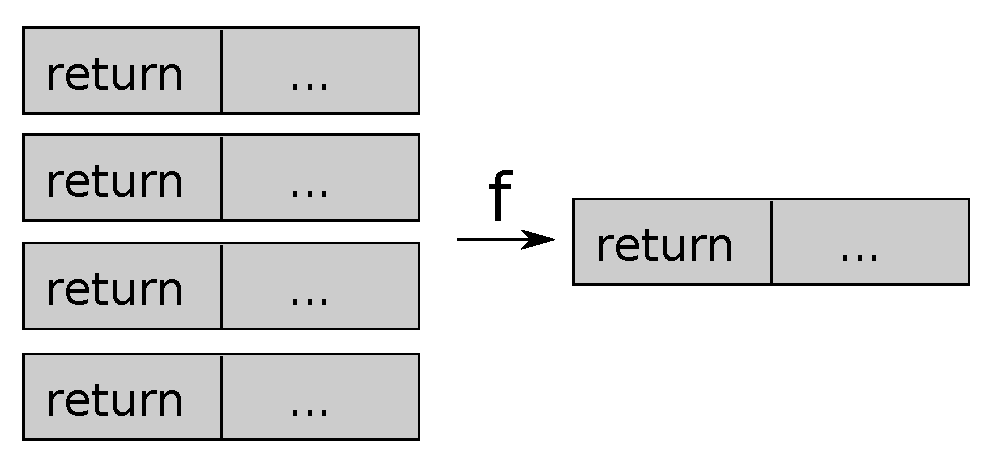
\includegraphics[height=100px]{purity-preservation}
%
%Ist nicht sichergestellt, dass sämtliche Elemente der Eingabeliste rein sind, kann man sich weiter überlegen, dass eine
%Möglichkeit zur Verfügung steht, mit der man den reinen Inhalt des monadischen Werts extrahieren kann - ähnlich wie
%die unsichere Funktion \texttt{unsafePerformIO}, die den reinen Wert aus einer IO-Monade extrahiert, nur eben für
%andere Monaden und sicher.
%Es ist ja vorstellbar, dass man nur am reinen Ergebnis einer Funktion $f$ interessiert ist, unabhängig von eventuellen anhaftenden
%monadischen Effekten. Tatsächlich kann man unter bestimmten Voraussetzungen zeigen, dass man beliebige Effekte in der 
%Eingabeliste ignorieren kann, wenn man nur am reinen Ergebnis interessiert ist.
%
%Sei $f :: Monad\ m \Rightarrow [m\ Int] \rightarrow m\ Int$, sei $\kappa$ eine Monadeninstanz und sei $p :: \kappa\ a \rightarrow a$, d.h. $p$ ist die erwähnte Funktion, die den reinen Wert aus dem monadischen Kontext extrahiert.
%Wenn folgende Aussagen gelten:
%
%\begin{itemize}
%\item $p \circ return_{\kappa} = id$
%\item Für beliebige Typen $t, t'$ und beliebige $m :: k\ t, k :: t \rightarrow k t'$ gilt\\
%$p (m\ {>>=}_{\kappa}\ k) = p\ (k\ (p\ m))$
%\end{itemize}
%
%dann liefert $p \circ f_{\kappa}$ das gleiche Eregbnis für beliebige Listen gleicher Länge, deren Elemente an jeweils gleicher Position
%die gleichen p-Bilder haben, sprich: den gleichen reinen Anteil. Man kann $p \circ f_{\kappa}$ kann also auch erhalten durch
%$g \circ (map\ p)$ für eine passende Funktion $g :: [Int] \rightarrow Int$ \cite{voigtlander}.
%
%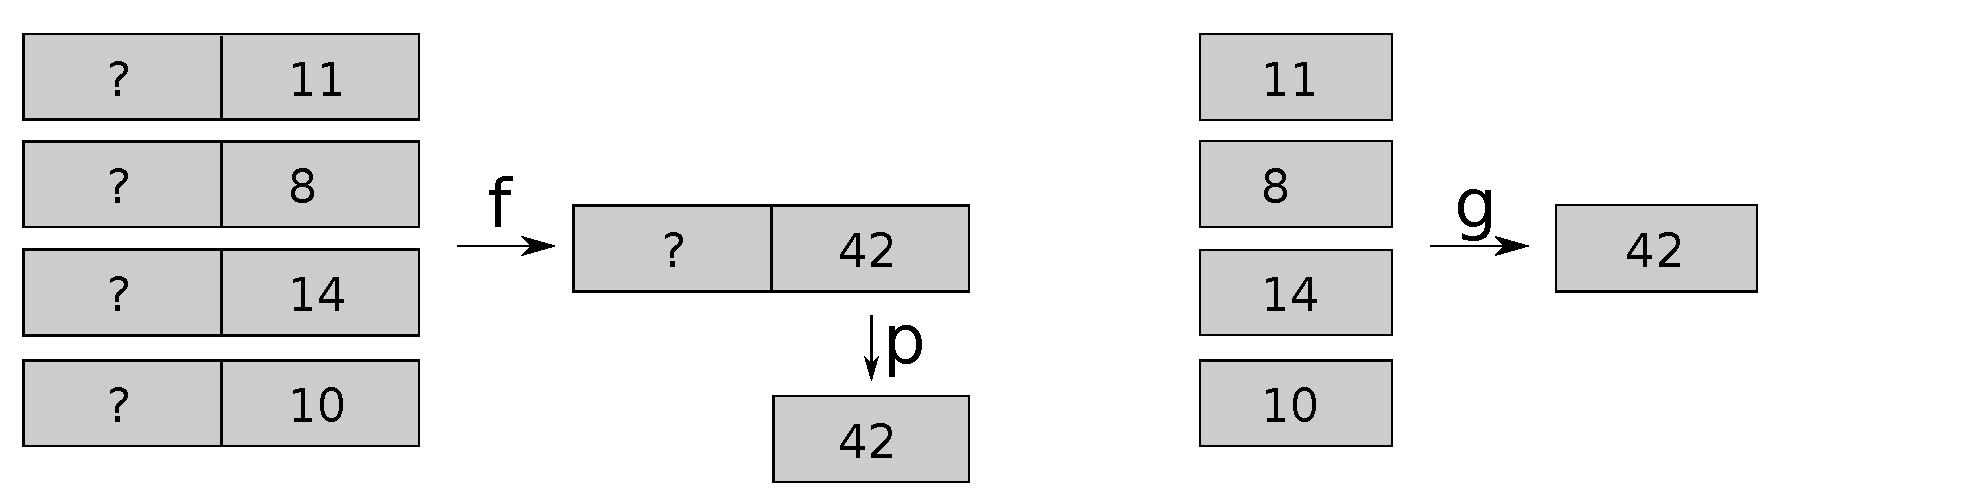
\includegraphics[height=100px]{safe-value-extraction}
%
%Für diese Aussage werden keine Monadengesetze benötigt.